
Scalar active systems are those whose large-scale dynamics is well captured by a real (scalar) field, hereafter denoted $\rho$. 
As we have seen in~\autoref{chap_intro}, the field $\rho$ is usually referred to as the \emph{order parameter} of the theory.
While it can in general represent various quantities related to the dynamics, here it will be most of time given by the particle density.

% At equilibrium, the minimal continuous description of scalar systems with conserved order parameter is achieved via \emph{model B} (see~\cite{HohenbergRMP} for a comprehensive classification).
% Model B indeed describes a class of equilibrium systems whose dissipative dynamics is captured by a conserved field, such that $\intd{r} \, \phi(\bm r,t) = {\rm const}$, for all times $t$,  where hereafter the variables $\bm r$ and $t$ account for space and time, respectively, while $d$ denotes the number of spatial dimensions.
% As model B describes the universal large-scale features of many systems, it can be formulated based on relevant symmetries and conservation laws.
% Such a phenomenological approach can moreover be supplemented by direct coarse-graining from microscopic (particle-based) theories, which provide additional physical insights. 

% In these notes, we will apply both approaches---phenomenological and coarse-graining---to study the dynamics of scalar active systems.
% We begin with a bottom-up approach
% In \autoref{chapter: introduction}, we introduced the active Brownian particle (ABP). 
% By extending this model to a collection of interacting ABPs, we will employ coarse-graining techniques to obtain one of the paradigmatic examples of collective active matter, motility-induced phase separation (MIPS).
% Here we will review some of the essentials of equilibrium phase separation physics, what changes for methods that do not admit an equilibrium description, and discuss what is needed for this to be the case.
% We will then take a more phenomenological approach to derive the Active Model B (AMB) and the Non-Reciprocal Cahn-Hilliard (NRCH) model, and explore their rich out-of-equilibrium features.



\section{Interacting active Brownian particles}

\subsection{The microscopic model}

In \autoref{intro_ABM}, we introduced a simple model of noninteracting active Brownian particles. 
Here, we consider the simplest extension of this model by assuming that we have isotropic particles that interact via volume exclusion. 
For simplicity, we restrict our analysis to two spatial dimensions, while most of what we present below also holds in $d=3$.

We thus have $N$ active particles defined by their positions $\bm r_i$ and self-propulsion orientations $\theta_i$, $i \in \{1, \dots N\}$.
As we have seen before, we can model their dynamics in terms of overdamped Langevin equations.
In two dimensions, these take the form
% The dynamics of each of these particles are described by an underdamped Langevin equation with an active velocity, as in \autoref{chapter: introduction}.
% Without interaction, it 
% %
% \begin{align}
%     \odv{\bm r_i}{t} = \bm v_{i,a}(t) + \sqrt{ 2 D_t } \bm \xi_i(t),
% \end{align}
% %
% where $\bm \xi_i(t)$ is white Gaussian noise, which obey
% %
% \begin{align}
%     \E{\xi_{k,i}(t)} &= 0, &
%     \E{\xi_{k,i}(t)\xi_{k',j}(t')} = \delta_{ij} \delta_{kk'} \delta(t - t').
% \end{align}
% %
% In two dimensions, the active velocity may be parametrized in terms of a single angle, $\bm v_a(t) = v_0 \hat {\bm e}(\theta(t))$, where 
% %
% \begin{align}
%     \hat {\bm e}(\theta) 
%     =
%     \begin{pmatrix}
%         \cos \theta \\ \sin \theta
%     \end{pmatrix}.
% \end{align}
%
%We focus on times much larger than the time scale of the rotational noise, $t\gg \tau_r = 1 / D_r$, so we may consider the rotational noise $\xi_i(t)$ to be white Gaussian noise as well.
%Including the interaction potential $U$, the full equations of motion for each particle becomes
%
\begin{subequations}
\label{eq_Langevin_int_ABPs}
\begin{align}
    \odv{\bm r_i}{t} & = v_0 \hat {\bm e}(\theta_i) - \frac{1}{\zeta} \nabla_{\bm r_i} U(\{\bm r_j\}) + \sqrt{ 2 D } \bm \xi_i, \\
    \odv{\theta_i}{t} & = \sqrt{ 2 D_r } \chi_i,
\end{align}
\end{subequations}
%
where $\zeta$ and $D$ correspond respectively to the friction and diffusivity, and are related by the relation $D = k_B T / \zeta$,
$D_r$ denotes the rotational diffusivity of the self-propulsion direction, while the unit vector parametrizing the direction of self-propulsion takes the form
%
\begin{align}\label{unit vector}
    \hat {\bm e}(\theta) 
    =
    \begin{pmatrix}
        \cos \theta \\ \sin \theta
    \end{pmatrix}.
\end{align}
%
As before, the noises in~\eqref{eq_Langevin_int_ABPs} are Gaussian with zero mean, uncorrelated, and satisfy
\begin{equation*}
    \E{\xi_{k,i}(t)\xi_{k',j}(t')} = \delta_{kk'}\delta_{ij} \delta(t - t'), \qquad
    \E{\chi_{k}(t)\chi_{k'}(t')} = \delta_{kk'} \delta(t - t'). 
    %\qquad k,k' \in \{1,\ldots,N\}, \quad i,j \in \{1,2\}.
\end{equation*}
The interactions between the particles are modeled via a potential $U$, which we assume has the form
%
\begin{align*}
    U(\bm r_1, ..., \bm r_n) = \sum_{i \neq j} u(|\bm r_i - \bm r_j|).
\end{align*}
%
In the following, we also assume that $u$ is short-ranged, isotropic and repulsive: two particles only interact when they are in contact, while the amplitude and direction of the resulting force only depend on the vector joining their centers of mass.
The simplest choice satisfying these criteria is the hard-core potential 
\begin{equation*}
    u_{\rm HC}(r) = \begin{cases} +\infty & {\rm if}\; r < d_0\\
        0 & {\rm otherwise} \end{cases} ,
 \end{equation*}
that prevents any overlap between the particles below the scale $d_0$ that plays the role of their diameter.
In practice---i.e. for simulations---the hard core potential is often approximated via the Weeks-Chandler-Andersen potential (or truncated Lehnnard-Jones potential):
\begin{equation*}
    u_{\rm WCA}(r) = \begin{cases} 4\epsilon\left[ \left(\frac{d_0}{r}\right)^{12} - \left(\frac{d_0}{r}\right)^{6} \right] + \epsilon & {\rm if}\; r < 2^{1/6} d_0\\
        0 & {\rm otherwise} \end{cases} .
 \end{equation*}
Alternatively, one can also allow finite overlaps between particles by using a softer repulsion potential.
A common choice is the harmonic repulsion:
\begin{equation*}
    u_{\rm soft}(r) = \begin{cases} \tfrac{\epsilon}{2}(1 - r/d_0)^2 & {\rm if}\; r < d_0\\
        0 & {\rm otherwise} \end{cases} .
 \end{equation*}
 All the aspects that we describe below are qualitatively independent of the details of the interaction potential, so we do not make any specific choice below. 

\begin{figure}[!t]
    \centering
    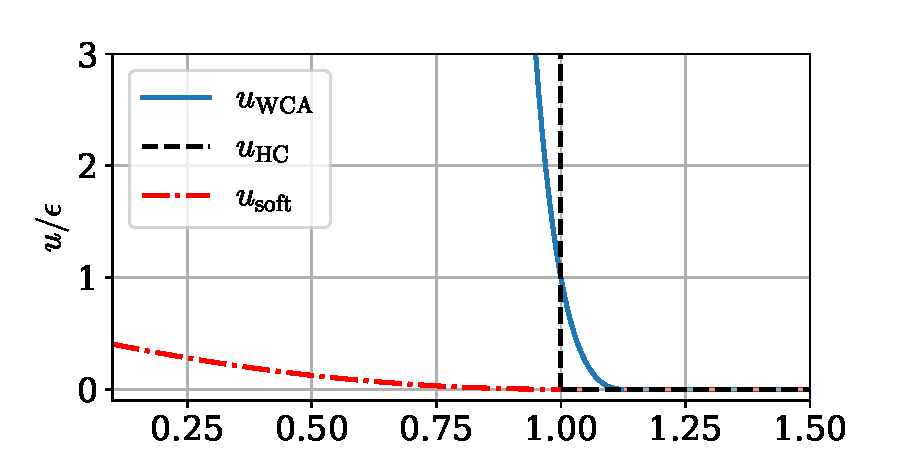
\includegraphics[width=.4\textwidth]{chapters/Figures/scalar/pot.pdf}
    \caption{Illustration of the possible choices for the potential $u$. A hard repulsion corresponds to $\lim_{r\to0} u(r) = +\infty$, so the particles can never fully overlap. For the soft repulsion the maximum value of the potential is finite, so overlaps are always possible.}
    \label{fig: hard soft}
\end{figure}


\subsection{Numerical simulations}

Rescaling space with the particle diameter $d_0$ and time with the typical rotational diffusion timescale $\tau_r = 1/D_r$, Eqs.~\eqref{eq_Langevin_int_ABPs} read in dimensionless coordinates
\begin{subequations}
\label{eq_Langevin_int_ABPs_ND}
\begin{align}
    \odv{\bm r_i}{t} & = {\rm Pe} \, \hat {\bm e}(\theta_i) - \frac{\epsilon\tau_r}{\zeta d_0^2} \nabla_{\bm r_i} U(\{\bm r_j\}) + \sqrt{ \frac{2 D\tau_r}{d_0^2} } \bm \xi_i, \\
    \odv{\theta_i}{t} & = \sqrt{ 2 } \chi_i,
\end{align}
\end{subequations}
where we have defined $\epsilon$ as the unit scale of energies, while ${\rm Pe} = v_0\tau_r / d_0$ is usually referred to as the \textit{Péclet number} and set the strength of activity.

\textit{
{\bf Homework:}
From the relation $\int_{-\infty}^{+\infty}\dd t \,  \delta(t) = 1$, show that the physical unit of $\delta(t)$ corresponds to the inverse of a time. 
Use this result to deduce how the noises in Eqs.~\eqref{eq_Langevin_int_ABPs} rescale in dimensionless coordinates, and recover Eqs.~\eqref{eq_Langevin_int_ABPs_ND}. 
}

In dimensionless coordinates, the strength of activity is therefore set by the ratio of the persistence length of the active motion and the interaction range.
Simulating Eqs.~\eqref{eq_Langevin_int_ABPs_ND} in the low activity regime (i.e., either at low $v_0$ and/or low $\tau_r$), 
the dynamics qualitatively corresponds to that of an equilibrium gas of repelling particles.
When activity is increased sufficiently, \autoref{fig: MIPS} shows that the particles spontaneously self-organize into a dense macroscopic domain coexisting with a surrounding dilute gas.
The densities of the dilute and dense phases are largely insensitive to variations of the mean particle density, which only set their relative volume fractions.
This phenomenology is thus similar to that of equilibrium phase separation.
Although the emergence of phase separation at equilibrium requires the presence of attractive interactions between the molecules,
here no explicit attractive interactions are present.
In fact, the cluster formation finds its origin in the interplay of activity and crowding effects.
This collective behavior is known as \textit{motility-induced phase separation} (MIPS), and we will spend the following sections to explain its emergence. 
For modern a review on MIPS that goes beyond the contents of this chapter, we recommend Ref.~\cite{bookMIPS2023}.

\begin{figure}[!t]
    \centering
    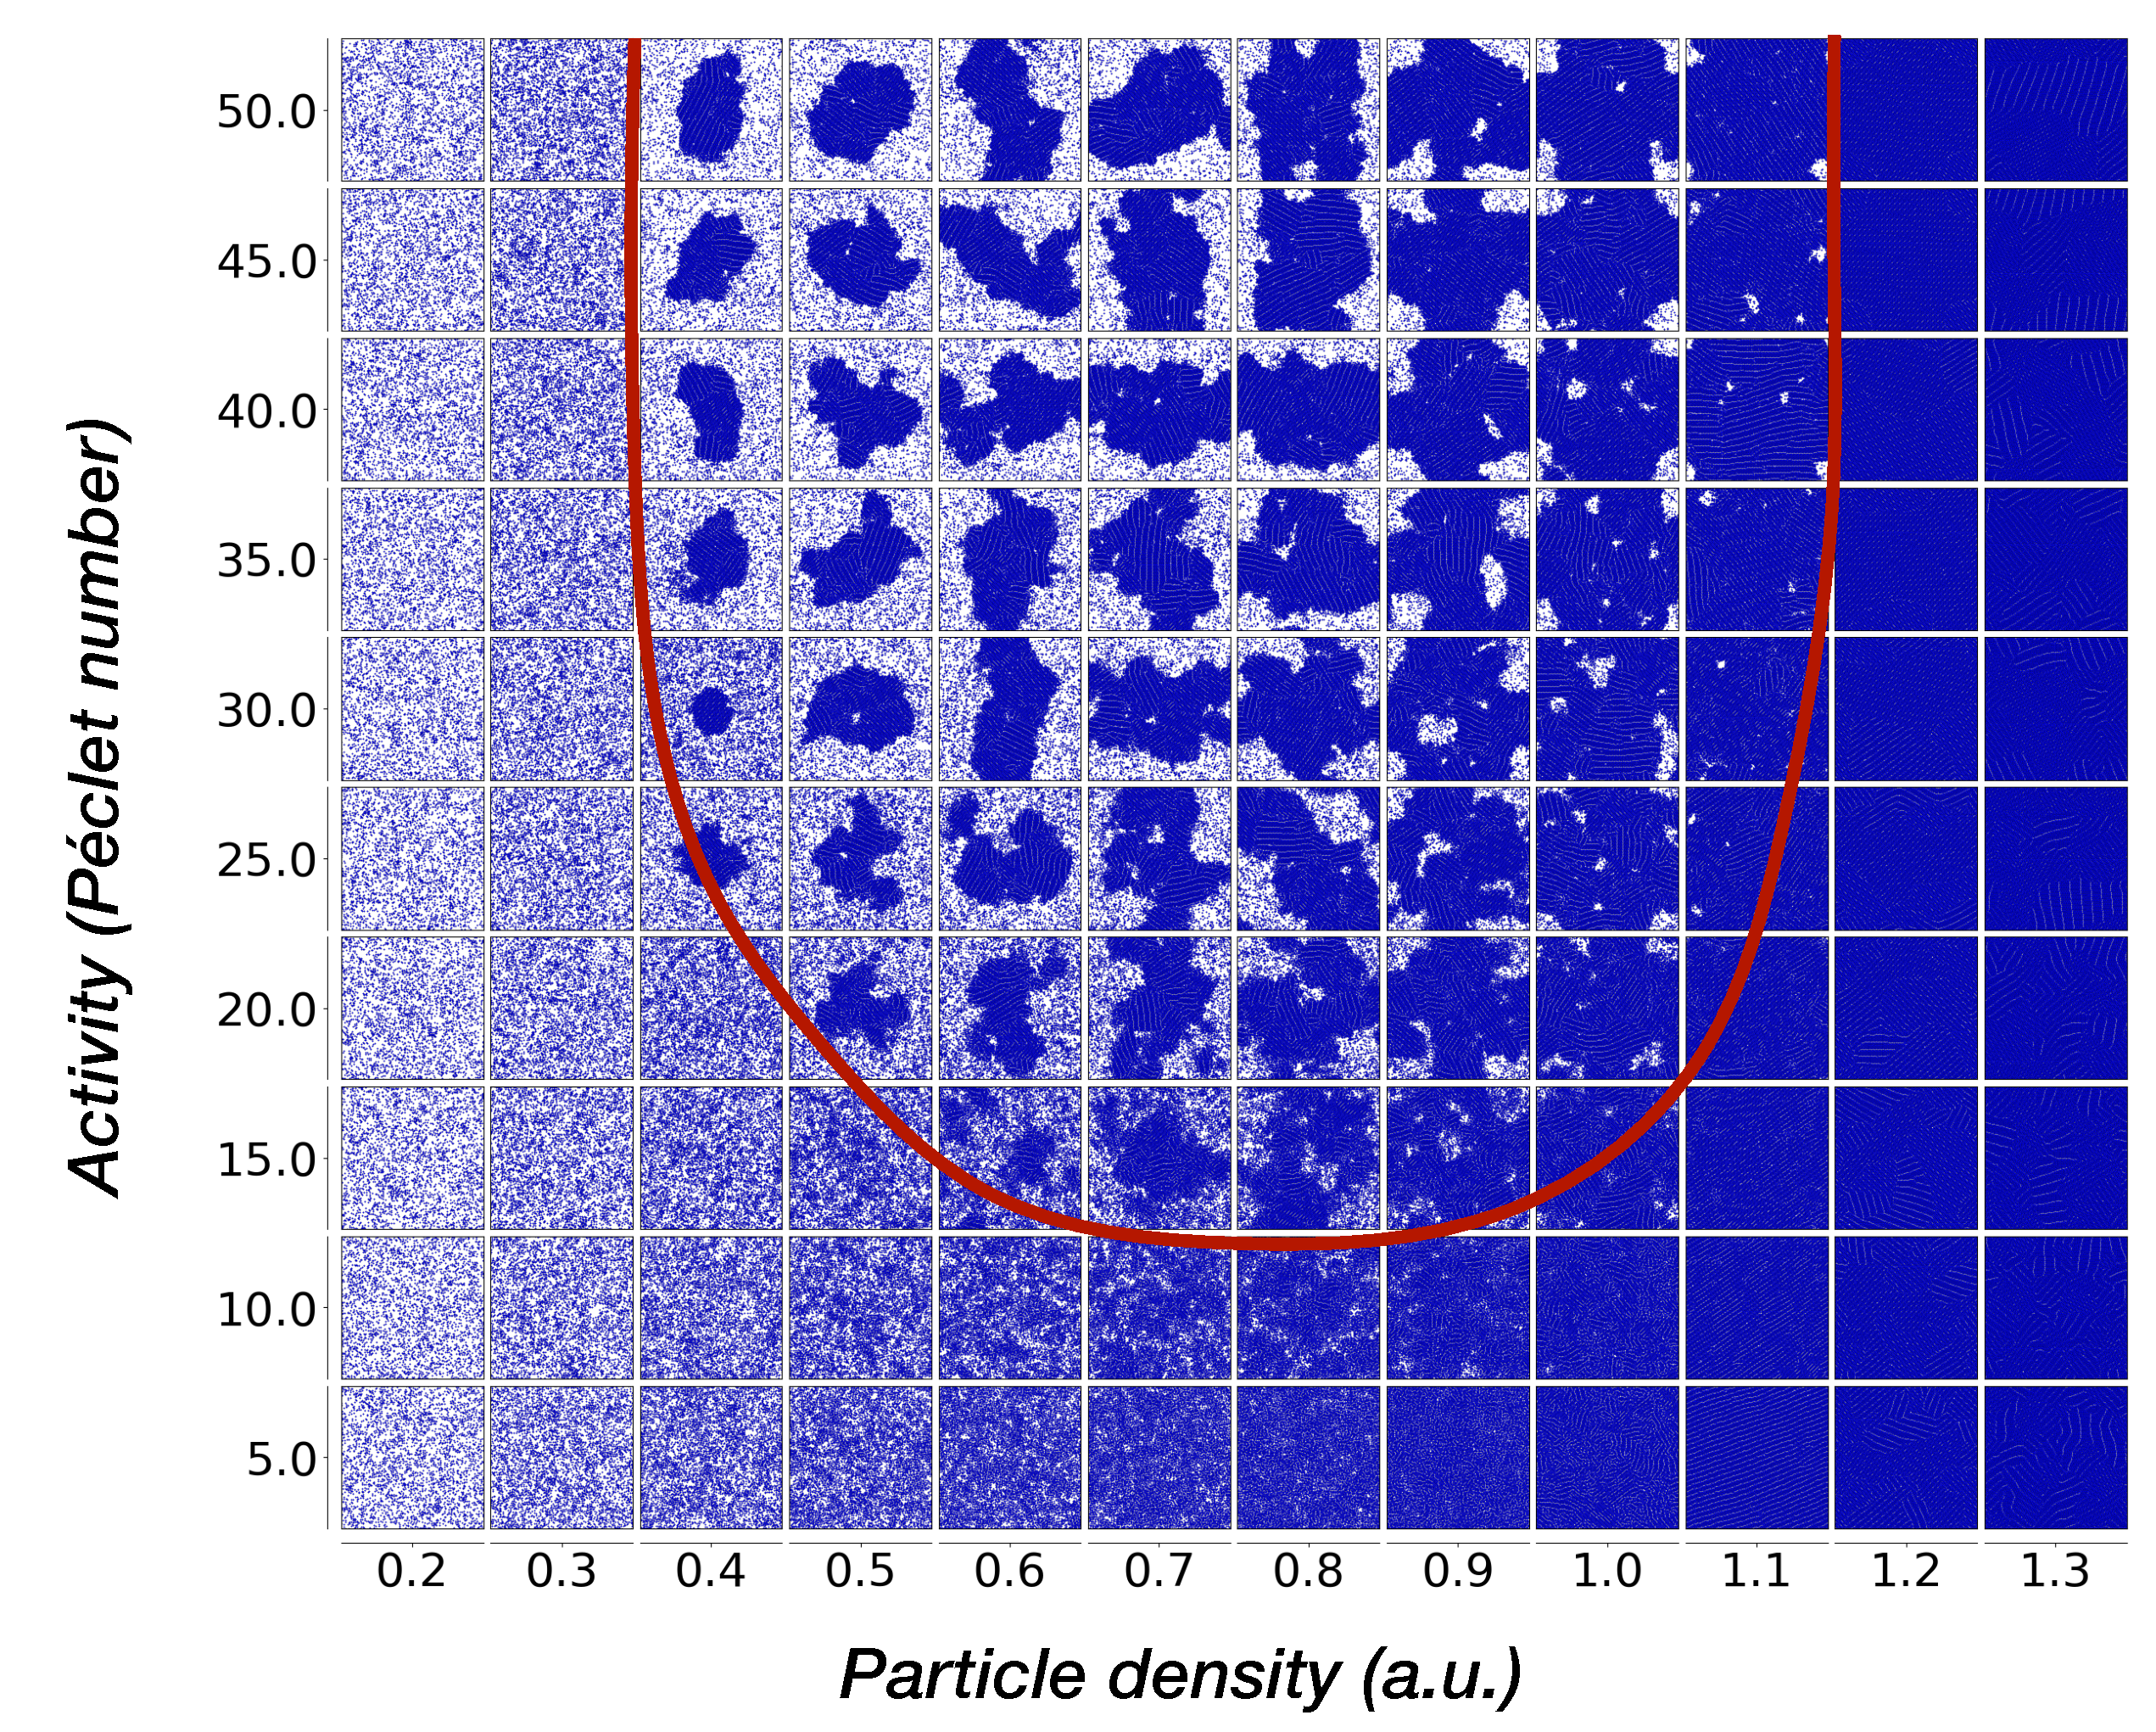
\includegraphics[width=.6\textwidth]{chapters/Figures/scalar/Fig_MIPS_PD.pdf}
    \caption{Phase diagram of the active Brownian particle model in the particle density - activity plane.
    Each panel shows a representative snapshot of the steady state configuration of the system.
    At large enough activity, the system undergoes a clustering instability, resulting in phase separated configurations where a dilute and a dense phase coexist.
    The red line serves as a guide for the eye to separate homogeneous and phase-separated configurations.
    \textit{Figure credits: Theo Spornhauer, University of Göttingen.}}
    \label{fig: MIPS}
\end{figure}

\subsection{The Mean field approach: a simple argument}

\label{sec_MF_simple_arg}

A minimal continuum model of equilibrium phase separation is the \textit{Cahn-Hilliard model}, that consists of a consereved Ginzburg-Landau-type dynamics of the particle density (see~\autoref{chapter: phase sep} for further details).
Since MIPS qualitatively resembles equilibrium phase separation, we expect that it can also be understood by an effective theory written in terms of the relevant field variable.
%As MIPS results from a many-body dynamics, it'll be better understood from a field theoretical description of the microscopic dynamics~\eqref{eq_Langevin_int_ABPs} expressed in terms of the relevant variables.
To derive such theory from the microscopic dynamics~\eqref{eq_Langevin_int_ABPs}, the usual procedure consist in writing its statistical description in terms of the $N$-body particle distribution distribution,
%
\begin{align} \label{eq_PN}
    \calP_N(\{\bm x_i, \phi_i\}, t) = \E{ \prod_i \delta(\bm r_i(t) - \bm x_i)\delta(\theta_i(t) - \phi_i) },
\end{align}
%
whose evolution is ruled by the Fokker-Planck equation.
Assuming the particles to be indistinguishable, the single-body particle distribution is then obtained by integrating over $3(N-1)$ degrees of freedom: 
$$\calP(\bm x,\phi,t) = N\int\prod_{j=2}^N [\dd\bm x_j \dd\phi_j]\,\calP_N(\{\bm x,\phi,\bm x_2,\phi_2,\ldots,\bm x_N,\phi_N\},t),$$
while the particle density $\rho(\bm x,t) = \int\dd\phi \calP(\bm x,\phi,t)$.
%The particle density $\rho$ is then obtained from the single-body distribution $\calP(\bm x,\phi,t) = N\int\prod_{j=2}^N [\dd\bm x_j \dd\phi_j]\calP_N(\{\bm x,\phi,\bm x_2,\phi_2,\ldots,\bm x_N,\phi_N\},t)$ as $\rho(\bm x,t) = \int\dd\phi \calP(\bm x,\phi,t)$.

If the particles are not interacting, the probability distribution~\eqref{eq_PN} simply factors into $N$ independent single-body distributions. 
On the other hand, interactions introduce non-trivial correlations which prevent such factorization.
In this case, the effective equation for the single-body distribution is a function of the two-body distribution, which itself depends on the three-body distribution, etc. 
Obtaining the effective theory for $\calP(\bm x,\phi,t)$ thus requires to solve the so-called Bogoliubov-Born-Green-Kirkwood-Yvon (BBGKY) hierarchy for all $n$-body distributions.
Doing this exatly is in general impossible, so that achieving analytical progress requires to use a number of approximations.
While we present a derivation of the effective dynamics for $\calP(\bm x,\phi,t)$ in~\autoref{appendxi: BBKGY}, here we will instead focus on describing the effective effect of the coupling between the particle self-propulsion and the repelling interactions by means of a mean field approximation.

Consider an isolated particle moving freely.
Its instantaneous self-propulsion speed is then given by $v_0$. 
If, on the other hand, our tagged particle enters a region of high density, it will begin to collide with other particles, the main result of which will be to reduce its effective self-propulsion speed.
To use a familiar analogy, imagine yourself running in an open field or within a crowd at a concert.
Using this simple reasoning, we can thus approximate the interactions in Eqs.~\eqref{eq_Langevin_int_ABPs} as an effective slowing down of the self-propelled motion when the particle density increases.
Therefore, we can simply discard the interaction potential and replace the constant self-propulsion speed with a $\rho$-dependent function:
%
\begin{align*}
    v_0 \rightarrow v(\rho), \qquad
    \odv{v}{\rho} = v'(\rho) \le 0.
\end{align*}
%
This way, we achieve a simpler description of the dynamics as it can now be expressed directly in terms of the single-body distribution $\calP$.
%In general, we may consider a self-propulsion speed dependent on space and time, $v = v(\bm x, t)$.

As a result of our mean field assumption, the particle self-propulsion speed is now a function of space.
Hence, to get some intuition on the behavior of the system let us first study the behavior of a single active particle in a landscape of spatially-dependent activity.
We thus set $v_0 \to v_0(\bm x)$ and $D = 0$ to keep things simple.
The dynamics is then described by the Fokker-Planck equation
\begin{align} \label{eq: space dependent fokker planck}
    \partial_t \calP(\bm x, \phi, t)
    + \bm \nabla \cdot [
        v_0(\bm x) \hat {\bm e}(\phi ) \calP(\bm x, \phi, t) ]
        - D_r \partial_\phi^2 \calP(\bm x, \phi, t)
        = 0.
\end{align}

Setting $\partial_t \calP = 0$, it is clear that the steady state solution of Eq.~\eqref{eq: space dependent fokker planck}
is isotropic: $\calP_{\rm s}(\bm r) = \rho_{\rm s}(\bm r)/2\pi$, which leads to
%
\begin{align} \label{eq_sol_rhos_landscape}
    \bm \nabla [v_0(\bm x)\rho_{\rm s}(\bm x)] = 0
    \implies 
    \rho_{\rm s}(\bm x) \propto \frac{1}{v_0(\bm x)}.
\end{align}
%
Equation~\eqref{eq_sol_rhos_landscape} confirms the intuition that particles will on average stay longer in regions where they are slower,
leading to a local increase of their density.
Therefore, activity landscape can be used to structure the density field of active systems. 
Experimentally, this can be realized, e.g., via photo-responsive colloids or genetically engineered bacteria~\cite{Arlt2018,Frangipane2018}, with density profiles that are consistent with the prediction~\eqref{eq_sol_rhos_landscape}.

We can now use this result to predict the emergence of MIPS. 
For this, let us consider an assembly of self-propelled particles with density-dependent self-propulsion $v(\rho)$ initially arranged in a configuration with uniform density $\bar\rho$.
Applying an infinitesimal perturbation such that $\rho(\bm x,t) = \bar \rho + \delta \rho(\bm x,t)$ with $\delta \rho \ll \bar\rho$,
the self-propulsion speed landscape is then modified according to $v(\rho) \approx v(\bar \rho) + v'(\bar \rho)\delta\rho$, as illustrated in \autoref{fig: perturb}/.
This new landscape itself leads to a new density profile, which after denoting the new perturbation $\delta\rho'$ can be calculated from Eq.~\eqref{eq_sol_rhos_landscape} as 
%
\begin{align*}
    \bar \rho + \delta \rho'
    = 
    \frac{c}{v(\bar \rho) + v'(\bar \rho)\delta \rho}
    \approx \frac{c}{v(\bar \rho)} \left( 1 - \frac{v'(\bar \rho) \delta \rho}{v(\bar \rho)} \right)
    =
    \bar\rho - \frac{\bar\rho v'(\bar \rho)}{v(\bar \rho)} \delta \rho 
    ,
\end{align*}
%
where $c$ is a constant set by the density normalization and we have replaced $\bar\rho = c/v(\bar\rho)$ in the last equality. 
If $\delta\rho'/\delta\rho > 1$, then the initial perturbation is amplified by the coupling between self-propulsion and particle density, and otherwise it is damped and the density will relax to the homogeneous configuration.
Therefore, the homogeneous state is unstable whenever
\begin{align*}
    \frac{\bar \rho v'(\bar \rho)}{v(\bar\rho)} < -1.
\end{align*}
Within our simple mean field picture, we thus find that MIPS generically occurs whenever the effective self-propulsion speed of the active particle decays sufficiently fast as their density increases,
in qualitative agreement with numerical simulations of the active Brownian particle model.

\begin{figure}[!t]
    \centering
    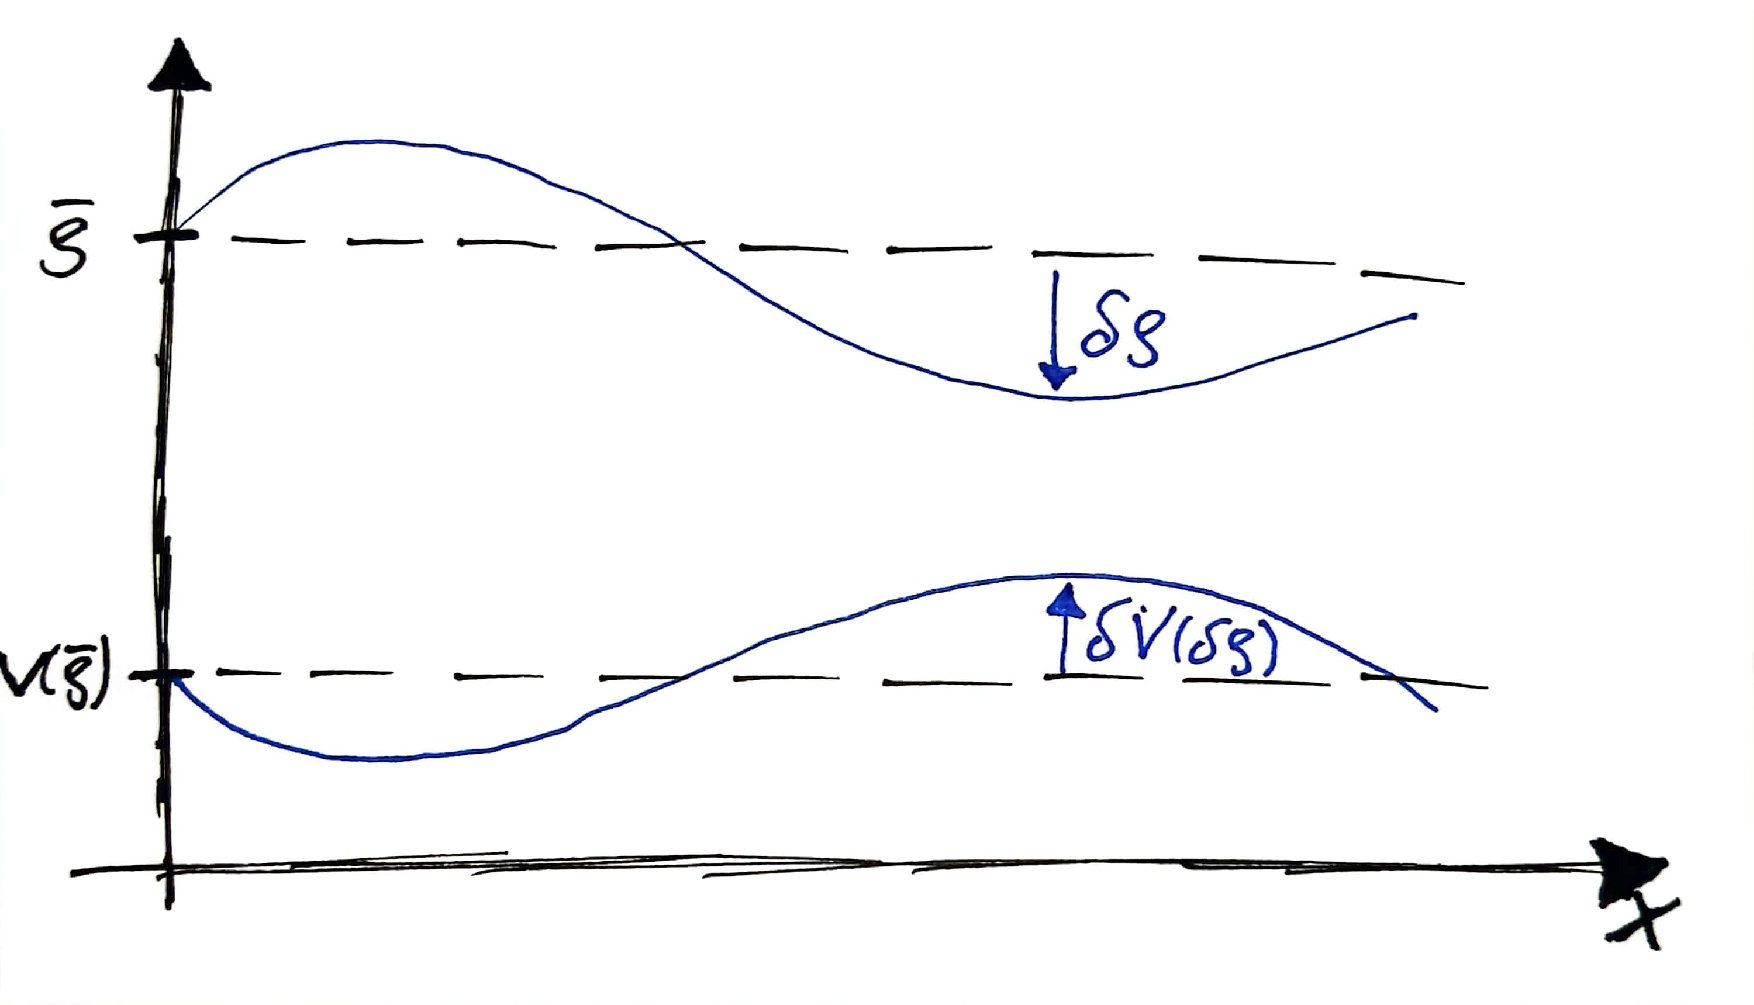
\includegraphics[width=.35\textwidth]{chapters/Figures/scalar/perturb.pdf}
    \caption{A perturbation of the density field around a homogeneous configuration induces a perturbed self-propulsion velocity landscape.}
    \label{fig: perturb}
\end{figure}


\subsection{The Mean field approach: moment expansion}

We now derive the above result  more rigorously.
For this, we first write the dynamics of the single-particle distribution as
\begin{align} \label{eq: density dependent fokker planck}
    \partial_t \calP(\bm x, \phi, t)
    + \bm \nabla \cdot [
        v(\rho) \hat {\bm e}(\phi ) \calP(\bm r, \phi, t)
        - D \bm \nabla \calP(\bm x, \phi, t)
    ]
        - D_r \partial_\phi^2 \calP(\bm x, \phi, t)
        = 0,
\end{align}
and where we have reintroduced positional diffusion for completeness.
Below, we derive the effective dynamics of the particle density field from~\eqref{eq: density dependent fokker planck} by means of a procedure called \emph{moment expansion}.

From its definition,
$\rho(\bm x, t) = \int_0^{2\pi} \dd \phi\, \calP(\bm x, \phi, t)$,
we obtain the equation for the density field by integrating Eq.~\eqref{eq: density dependent fokker planck} over $\phi$.
This yields
%
\begin{align}\label{eq: density FP}
    \partial_t \rho(\bm x, t)
    = 
    - \nabla \cdot [ v(\rho) \rho(\bm x, t) \bm p(\bm x, t) - D \nabla \rho(\bm x, t)],
\end{align}
%
where we have defined
\begin{align*}
    \rho(\bm x, t) \bm p(\bm x, t) =
    \int_0^{2\pi} \dd \phi \, \hat {\bm e}(\phi) \calP(\bm x, \phi, t),
\end{align*}
as the first moment of the distribution $\calP$ w.r.t.\ the particle orientation.
$\bm p$ measures how much the self-propulsion orientations of the particles are aligned locally, and is usually referred to as the polarity, or the polar field.
If $\calP(\bm x,\phi,t)$ is uniform in $\phi$, then from the expression of $\hat {\bm e}$, Eq.~\eqref{unit vector}, it is easy to show that $\bm p = \bm 0$.
On the other hand, if $\calP(\bm x,\phi,t)$ is strongly peaked around some angle $\phi_0$, so that $\calP(\bm x, \phi, t) \simeq \delta(\phi - \phi_0)$, then $\bm p \simeq \hat{\bm e}(\phi_0)$ (see \autoref{fig: polar and nematic} for an illustration).
Multiplying Eq.~\eqref{eq: density dependent fokker planck} with $\hat{\bm e}$ and integrating over $\phi$, we then get (in coordinates):
\begin{align} \label{eq: polarity FP}
    \partial_t [\rho(\bm x, t) p_i(\bm x, t)]
    = - \partial_{j}
    \left\{
        v(\rho) \left[ \rho(\bm x, t) Q_{ij}(\bm x, t) + \frac{ \rho(\bm x, t) }{ 2 }  \delta_{ij}\right]
        - D \partial_j [\rho(\bm x, t) p_i(\bm x, t)]
    \right\}
    - D_r \rho(\bm x, t) p_i(\bm x, t),
\end{align}
where $\partial_i = \partial/\partial_{x_i}$ and summation over repeated indices is implied.
The equation for the polarity depends on the second order moment 
%
\begin{align*}
    \rho(\bm x, t) Q_{ij}(\bm x, t)
    = \int_0^{2 \pi} \dd \phi
    \left[
        \hat e_i(\phi)\hat e_j(\phi) - \frac{1}{2} \delta_{ij}
    \right] \calP(\bm x, \phi, t).
\end{align*}
%
While the polar order parameter $\bm p$ measures the alignment of small arrows, 
$\bm Q$ remains identical under the transformation $\hat{\bm e} \to -\hat{\bm e}$,
so that it measures by how much the orientations are aligned along the same axis, regardless of their direction, as illustrated in~\autoref{fig: polar and nematic}.
Note that $\bm Q$ is a rank-two tensor, and is usually called the \textit{nematic order}. 
%When half of the particles points in direction $\theta = 0$, while the rest points in the opposite direction $\theta = \pi$, the $p_i = 0$, while $Q\neq 0$.
%In fact, 
%
% \begin{equation}
%     Q = 
%     \begin{pmatrix}
%         1 & 0 \\ 0 & -1
%     \end{pmatrix}.
% \end{equation}
%
% General, higher-order moments describe the alignment of objects invariant under shorter and shorter rotations.
% The polar order parameter is invariant under a $2 \pi$ rotation, the nematic under a $\pi$ rotation, and so on.\footnote{
%     In quantum mechanics, we must also include fields that pick up a minus sign under rotations by $2 \pi / n$.
%     These are fermionic fields, while the fields introduced here are boson fields.
% }
% The difference between polar and nematic ordering is shown in \autoref{fig: polar and nematic}

\begin{figure}[!b]
    \centering
    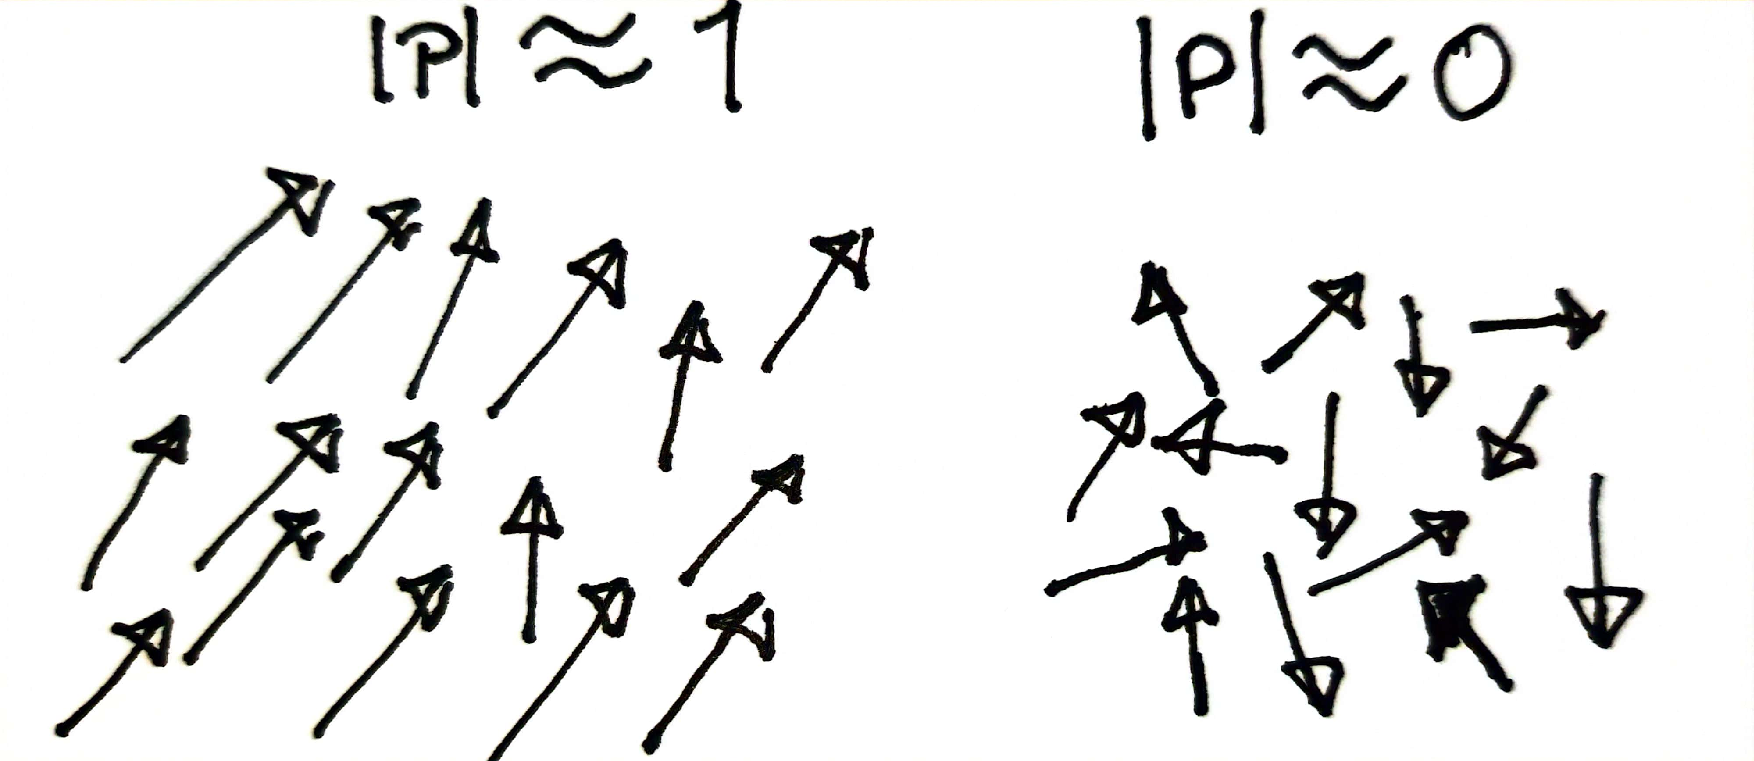
\includegraphics[width=.38\textwidth]{chapters/Figures/scalar/polar.pdf}
    \hspace{1cm}
    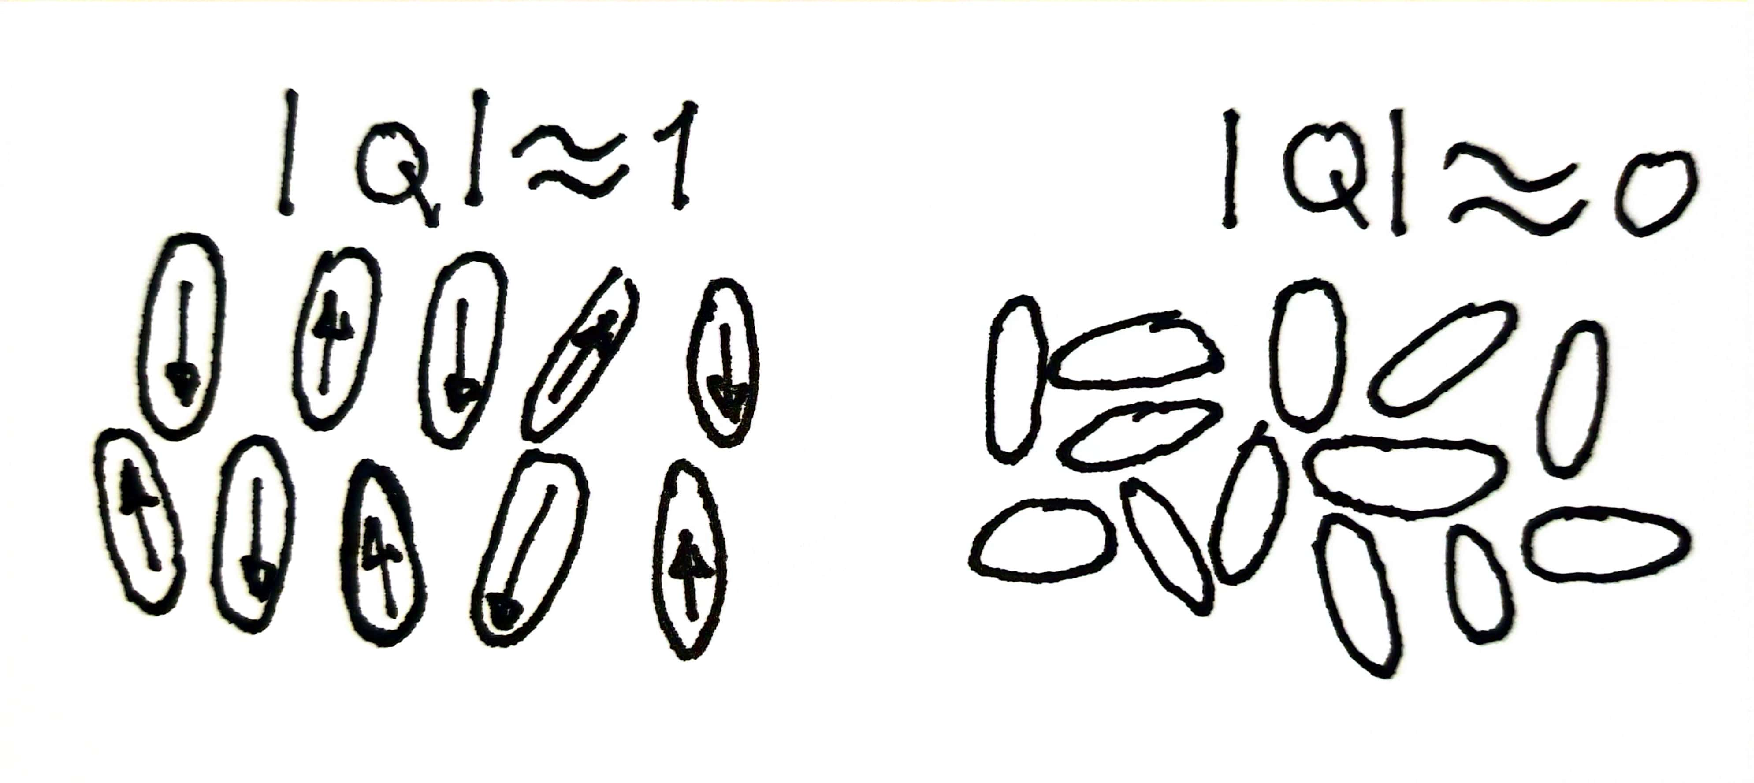
\includegraphics[width=.4\textwidth]{chapters/Figures/scalar/nematic.pdf}
    \caption{
    On the left: like the magnetization, the polar order measures the ordering of arrows.
    On the right: the nematic order is not sensitive to the direction of the arrows but only to their orientation. Hence, configurations that remain statistically identical when all arrows are flipped still present high a nematic order.}
    \label{fig: polar and nematic}
\end{figure}

\textit{{\bf Homework:} From its definition, show that the nematic order is traceless (${\sum}_i Q_{ii} = 0$).
By calculating the expression of $\bm Q$ for a uniform distribution of orientations, explain why.}

It should appear clear by now that the equation satisfied by $\bm Q$ will depend on higher order moments of the orientation, so that the hierarchy of moments is infinite.
Below, we thus close it by relying on controlled approximations. 
First, we note that, as a consequence of the fact that the density is a conserved field, the r.h.s.\ of Eq.~\eqref{eq: density FP} corresponds to the divergence of a current.
Therefore, the typical timescale $\tau_\rho$ associated with the relaxation of $\rho$ is set by mass transport, and depends on the length scale of interest. 
In practice, we thus assume that $\tau_\rho \sim \nabla^{-\alpha} \sim L^\alpha$,
with $L$ the length scale of interest and $\alpha$ a positive exponent.
On the other hand, the dynamics of $\rho\bm p$ includes a linear damping term $-D_r \rho\bm p$.
This damping term originates from the fact that rotational diffusion randomizes the orientations, so that the equations for all higher order moments share a similar structure as~\eqref{eq: polarity FP}.
Hence, any perturbation of these moments relaxes on a finite timescale $\tau_r \simeq 1/D_r$ regardless of the associated length scale.

On large enough length scales,
the density thus evolves over a timescale $\tau_\rho \gg \tau_r$,
so that $\rho$ is the only relevant field variable to consider if one is interested in describing the macroscopic physics.
In the language of statistical physics, $\rho$ is usually referred to as a \emph{slow mode} or a \emph{hydrodynamic mode}.
As we have studied in~\autoref{chap_intro}, hydrodynamic modes can also originate from non-conserved dynamics, e.g. when a continuous symmetry is spontaneously broken. 

\textit{{\bf Homework:} Using the divergence theorem, show that if a field $\rho$ obeys an equation of the form $\partial_t \rho + \nabla \cdot \bm J = 0$ with $\bm J$ the corresponding current, then for an isolated system of volume $V$ the total mass $m = \int_V\dd\bm x \, \rho(\bm x,t)$ is conserved.}

In addition, we assume that the fields are sufficiently smooth so that we perform an expansion in gradients.
Keeping only the leading order terms in Eq.~\eqref{eq: polarity FP}, we discard the term $\nabla^2(\rho\bm p)$. 
Moreover, from the equation of the nematic order it straightforward to show that, at leading order, $\rho Q_{ij} \sim \partial_i [\rho v(\rho) p_j]$.
Discarding the corresponding contribution in Eq.~\eqref{eq: polarity FP}, 
we are left with
\begin{align*}
    \partial_t (\rho \bm p) + D_r \rho \bm p
    = - \frac{1}{2}\nabla[v(\rho) \rho].
\end{align*}
This equation can be solved exactly as
%
\begin{align}
    \rho(\bm x, t) \bm p(\bm x,t)
    = e^{- t D_r} \left\{ \rho(\bm x, 0) \bm p(\bm x,0) - \frac{1}{2}\int_0^t \dd t' \, e^{t' D_r} \nabla\left[v(\rho(\bm x,t'))\rho(\bm x,t')\right] \right\}.
\end{align}
%
As the first term on the r.h.s.\ vanishes exponentially fast in the limit $D_r t \gg 1$, we obtain after operating the change variables $\tau = t - t'$:
%
\begin{align*}
    \rho(\bm x, t) \bm p(\bm x, t)
    & = -\frac{1}{2} \int_{0}^t \dd \tau \, e^{- \tau  D_r} \nabla\left[v(\rho(\bm x,t-\tau))\rho(\bm x,t-\tau)\right]\\
    & =
    -\frac{1}{2} \int_0^\infty \dd \tau \, e^{- \tau  D_r} \left\{
    \nabla\left[v(\rho(\bm x,t))\rho(\bm x,t)\right]
    -\tau \partial_t \nabla\left[v(\rho(\bm x,t))\rho(\bm x,t)\right]
    + ...
    \right\}\\
    & \approx -\frac{1}{2 D_r} \nabla\left[v(\rho(\bm x,t))\rho(\bm x,t)\right],
\end{align*}
%
where in the second line we have used that $t D_r \gg 1$ to extend the upper bound of the integration range to infinity, 
while the last step was obtained by assuming that $\rho$ is almost stationnary over the time scale $\tau_r = 1 / D_r$.

The dynamics of $\bm p$ is now completely determined by, or enslaved to, the dynamics of the slow field $\rho$.
Replacing $\bm p$ by its expression in Eq.~\eqref{eq: density FP}, we finally obtain
\begin{equation} \label{eq_reduced_rho_ABP}
    \partial_t\rho = \nabla \cdot \left[
    D\nabla\rho + \frac{v(\rho)}{2 D_r}\nabla[v(\rho)\rho]
    \right].
\end{equation}
Equation~\eqref{eq_reduced_rho_ABP} describes the dynamics of the particle density over long times and large scales.
In fact, recovering the regime of constant self-propulsion speed with $v(\rho) \to v_0$ the density dynamics follows a diffusion equation with effective diffusivity $D_{\rm eff} = D + v_0^2/(2 D_r)$, which corresponds exactly to the result we derived in~\autoref{chap_intro} from the Langevin dynamics.

% A sanity check is to now substitute back in the special case $v(\rho) = v_0$, corresponding to non-interacting ABPs.
% The polar order-parameter is then given by
% %
% \begin{align}
%     \rho \bm p = - \frac{v_0}{2 D_R} \bm \nabla \rho,
% \end{align}
% %
% which when substituted back into Fokker-Planck for the density, \autoref{eq: density FP}, gives
% %
% \begin{align}
%     \partial_t \rho &= D_{\mathrm{eff}} \nabla^2 \rho, &
%     D_{\mathrm{eff}} = D + \frac{v_0^2}{2 D_R},
% \end{align}
% %
% which is excatly what we found in \autoref{chapter: introduction}.

% \textit{{\bf Homework}:
% In two dimensions, the vector $\he(\theta) = (\cos\theta, \sin\theta)$ is parametrized by the angle $\theta_t$. Assuming that $\theta_t$ is a Markov process, justify why we can write the joint distribution as $P(\theta_2,t_2;\theta_1,t_1) = P(\theta_2-\theta_1,t_2-t_1|0,0)P(\theta_1,t_1)$ for $t_2 > t_1$.
% Deduce that
% \begin{equation*}
%     \langle \he(\theta_t) \cdot \he(\theta_{t+\tau}) \rangle = \int \rmd\phi \cos\phi \, P(\phi,\tau|0,0) \equiv \langle \cos\phi \rangle_0, 
% \end{equation*}
% where $P(\theta,t)$ is the distribution of $\theta$ satisfying $P(\theta,0) = \delta(\theta)$.
% (Hint: Use the properties of $\theta$ to express the joint distribution $P(\theta_2,t_2;\theta_1,t_1)$)
% }


\subsection{The equilibrium mapping and emergence of MIPS}

With Eq.~\eqref{eq_reduced_rho_ABP}, we are in good position to study the emergence of phase separation.
In fact, we can recast the density dynamics as $\partial_t \rho(\bm x, t)  + \nabla \cdot \bm J[\rho(\bm x, t)]$ = 0,
where the associated current takes the form:
% 
\begin{align}\label{eq_J_ABP_MF}
   \bm J[\rho] = - \rho M(\rho) \nabla \mu(\rho).
\end{align}
%
Here, we have introduced the mobility $M(\rho) = D + v^2(\rho)/ (2D_r)$,
while density currents are induced by gradients of a generalized chemical potential 
\begin{align*}
    \mu(\rho) = \ln(\rho)
    + \int^{v(\rho)} \dd x \, \frac{x}{2 D D_r + x^2} = \ln\left[\rho \sqrt{2 D D_r + v^2(\rho)}\right].
\end{align*}
The expression of the current~\eqref{eq_J_ABP_MF} thus allows us to map the large scale behavior of active Brownian particles to an effective equilibrium dynamics described by a free energy $f(\rho)$, which we obtain up to some constant from as
%
\begin{align} \label{eq_eff_FE_ABPS}
    \mu(\rho) = f'(\rho) \implies
    f(\rho) = \int^\rho \dd x \, \ln \left[ x \sqrt{2 D D_r + v^2(x)}\right].
\end{align}
%
We can now directly apply methods developed to study phase separation at equilibrium, which are summarized in~\autoref{chapter: phase sep}.
Namely, considering a homogeneous density profile $\rho = \bar\rho$, 
we deduce from the equilibrium mapping 
that it will be unstable to small perturbations when the second derivative of the generalized free energy $f''(\bar{\rho})$ is negative.
Using Eq.~\eqref{eq_eff_FE_ABPS}, we find that this condition translates to
%
\begin{align} \label{eq_spinodal_ABPs}
    \frac{v(\bar \rho)v'(\bar \rho)\bar \rho}{2D D_r + v^2(\bar \rho)} < - 1.
\end{align}
%
Note that taking $D = 0$, we recover the criterion derived in~\autoref{sec_MF_simple_arg} from the simple argument.
Equation~\eqref{eq_spinodal_ABPs} defines
the limit of stability of homogeneous configuration, which correspond to the \emph{spinodal} curve of equilibrium phase separation.

When the system phase separates, we can moreover calculate the densities of the dense and dilute phases from the common tangent (or Maxwell) construction.
As detailed in~\autoref{chapter: phase sep}, diffusive and mechanical equilibria impose that the two phases have equal chemical potential and pressure, respectively.
In terms of the phase densities $\bar{\rho}_{1,2}$, these conditions read 
%
\begin{align} \label{eq_binodals_ABPS}
    \mu = f'(\bar \rho_1) = f'(\bar \rho_2), \qquad \qquad
    -P = f(\bar \rho_1) - \mu \bar\rho_1  &= f(\bar \rho_2) - \mu \bar\rho_2.
\end{align}
%
The two conditions in~\eqref{eq_binodals_ABPS} define a common tangent to the free energy curve $f(\rho)$ at the densities $\bar\rho_1$ and $\bar\rho_2$.

\autoref{fig: MF MIPS} shows a typical mean field phase diagram obtained from a specific choice of $v(\rho)$.
The binodals enclose the spinodals, such that the two curves only coincide at the critical point.
Hence, in some regions of the phase diagram phase separated configurations exist (and are stable) but the homogeneous state at $\rho = \bar\rho$ is also stable to small perturbations.
In practice, if we re-introduce noise into the dynamics, the homogeneous state will typically disappear 
not by the deterministic growth of an infinitesimal perturbation, but due to stochastic nucleation events that correspond to large disturbances and therefore cannot be captured by a linear stability analysis.
At sufficiently large activity and for $\bar\rho$ lying within the binodals, the system always phase separates over long times into two distinct domains 
with densities $\bar\rho_{1} \le \bar\rho_2$ and volumes ${\cal V}_{1,2}$.
Taking into account mass and volume conservation, the volumes of the two phases are given by
\begin{equation}
{\cal V}_1 = \frac{\bar\rho_2 - \bar\rho}{\bar\rho_2 - \bar\rho_1} {\cal V}, \qquad {\cal V}_2 = {\cal V} - {\cal V}_1 = \frac{\bar\rho - \bar\rho_1}{\bar\rho_2 - \bar\rho_1} {\cal V},
\end{equation} 
which is known as the \emph{lever rule}.

\begin{figure}[!t]
    \centering
    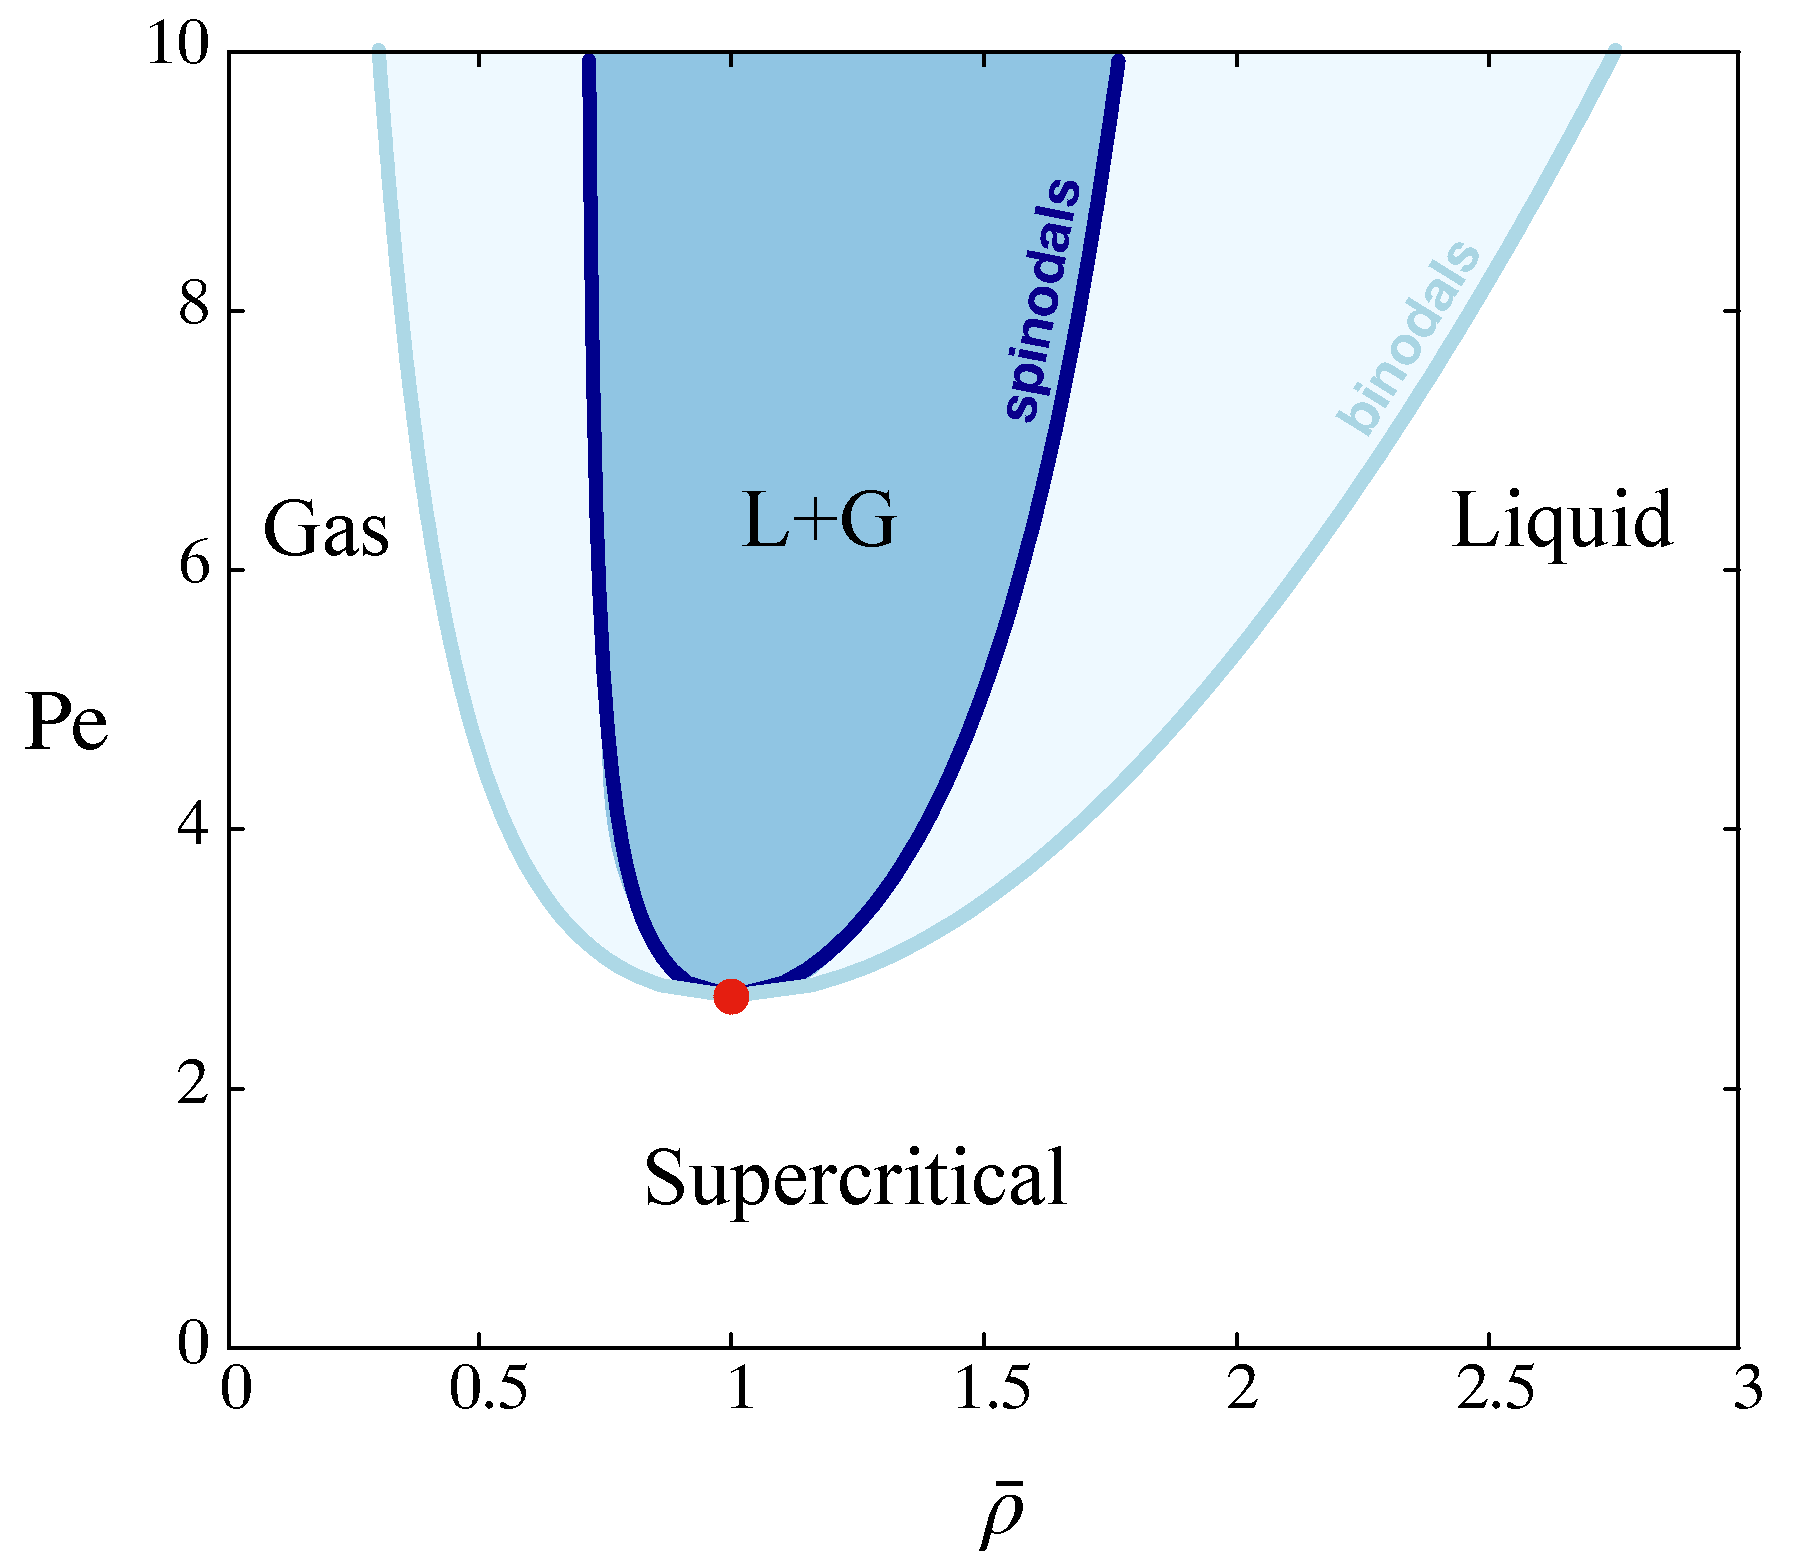
\includegraphics[width=.5\textwidth]{chapters/Figures/scalar/Fig_MF_MIPS.pdf}
    \caption{Mean field phase diagram of the active Brownian particle model for a density-dependent self-propulsion speed $v(\rho) = v_0 \exp(-\rho^2)$.
    The dark blue curve marks the spinodal densities computed from the condition~\eqref{eq_spinodal_ABPs}, while the light blue curve are the binodals obtained from~\eqref{eq_binodals_ABPS}.
    The red dot indicates the critical point.
    }
    \label{fig: MF MIPS}
\end{figure}

\textit{
{\bf Homework:}
The calculation detailed in~\autoref{appendxi: BBKGY}, as well as direct measurements from numerical simulations, suggest that the effective self-propulsion speed of the active particles decays linearly with the density:
\begin{align} \label{eq_linear_veff}
    v(\rho) = v_0(1 - \omega \rho)\Theta(1 - \omega\rho),
\end{align}
where $\Theta(x)$ is the Heaviside step function that is equal to one if $x \ge 0$, and zero otherwise.
\begin{enumerate}
    \item Show that, assuming the density-dependency~\eqref{eq_linear_veff}, the spinodal curve is defined by
    \begin{equation*}
        {\rm Pe} = \sqrt{\frac{2 \tilde D}{(1-\omega\bar\rho)(2\omega\bar\rho-1)}},
    \end{equation*}
    with the dimensionless parameters ${\rm Pe} = v_0/(D_r d_0)$ and $\tilde D = D / (d_0^2 D_r)$. Deduce that the region where spinodal decomposition occurs is restricted to $\tfrac{1}{2} < \omega\bar\rho < 1$, and calculate the coordonates of the critical point in the $(\bar\rho,{\rm Pe})$ plane.
    The generalized free energy describing the mean field dynamics is given by
    \begin{align*}
        f(\rho) = \rho\left[\ln\left(\rho\sqrt{2\tilde D}\right) - 1\right] + \Theta(1 - \omega\rho)\left[ \frac{1 - \omega\rho}{\omega}\left( 1 - \ln \sqrt{1 + \frac{{\rm Pe}^2(1-\omega\rho)^2}{2\tilde D}}\right) - \frac{\sqrt{2\tilde D}}{\omega {\rm Pe}}\arctan\left( \frac{{\rm Pe}(1-\omega \rho)}{\sqrt{2\tilde D}} \right) \right].
    \end{align*}
    You can check this directly by calculating $f'(\rho)$.
    \item In the vicinity of the critical point $(\rho_c,{\rm Pe}_c)$, show that $f(\rho)$ simplifies to
    \begin{equation*}
        f(\phi) = \frac{2}{3}\rho_c\phi^2\left( - \tilde{\rm P}{\rm e} - \frac{1}{3}\tilde{\rm P}{\rm e}\phi + \frac{3}{4}\phi^2 \right),
    \end{equation*}
    with $\phi = (\rho - \rho_c)/\rho_c$ and $\tilde{\rm P}{\rm e} = ({\rm Pe} - {\rm Pe}_c)/{\rm Pe}_c$.
    Draw $f(\phi)$ for $\tilde{\rm P}{\rm e} < 0$ and $\tilde{\rm P}{\rm e} > 0$, and explain why the common tangent construction will always give $\bar\phi_1 = \bar\phi_2 = 0$ for $\tilde{\rm P}{\rm e} < 0$.
    Show that for $\tilde{\rm P}{\rm e} > 0$ in the vicinity of the critical point the binodal densities satisfy
    \begin{equation*}
        \bar\phi_{1,2} \simeq \pm \sqrt{\frac{2}{3} \tilde{\rm P}{\rm e}}.
    \end{equation*}
    \item We now determine the behavior of the binodals in the limit of large activity.
    Assuming that, for $\rm Pe \to \infty$, $\bar\rho_1 \to 0$ and $\bar\rho_2 \to \infty$, show that
    \begin{align*}
        f(\bar\rho_1) & \simeq \bar\rho_1\left[\ln\left(\bar\rho_1\sqrt{2\tilde D}\right) - 1\right] 
        + \frac{1 - \omega\bar\rho_1}{\omega}\left( 1 - \ln\frac{\rm Pe}{\sqrt{2\tilde D}}\right) , \\
        f(\bar\rho_2) & \simeq \bar\rho_2\left[\ln\left(\bar\rho_2\sqrt{2\tilde D}\right) - 1\right].
    \end{align*}
    Then, deduce that 
    \begin{equation*}
        \bar\rho_1 \simeq \frac{\sqrt{2\tilde{D}}}{\omega{\rm Pe}}\left( \ln\frac{\rm Pe}{\sqrt{2\tilde D}} - 1\right), \qquad \bar\rho_2 \simeq \frac{{\rm Pe}}{\sqrt{2 \tilde D}}\bar\rho_1.
    \end{equation*}
    \item Using the answers to the previous sections, draw the phase diagram of the model in the $(\bar\rho,{\rm Pe})$ plane in the style of~\autoref{fig: MF MIPS}.
\end{enumerate}
}

% This is called motility-induced phase-separation, as the mechanism of phase is not attraction, as in passive systems, but a lowering of the motility in high densities.
% The mechanics of phase separation are thus non-equilibrium, however, the resulting large-scale dynamics are still described by an effective equilibrium theory.
% This comes as we can always find free energy, no matter the shape of $v(\rho)$.
% To break equilibrium also at the large scale, we must have a more general current.
% One way to obtain this is to extend the momentum expansion to higher orders.


\section{Breakdown of the equilibrium mapping: Active model B}

It may sound surprising at first that we managed to map a collective active dynamics to an effective equilibrium theory.
Actually, this feature is a simple consequence of the fact that we have expressed the current~\eqref{eq_J_ABP_MF} keeping only the terms at leading order in gradients.
Indeed, any smooth function $\mu(\rho)$ can be written as the derivative as another function $f(\rho)$, so that it is always possible to define an effective bulk free energy for the system.
At higher order in the gradient expansion, however, the situation is quite different.

To highlight this, let us consider the case where the effective self-propulsion speed is no more set by the local density, but by some local integral:
\begin{equation*}
    v(\rho) \to v(\tilde\rho), \qquad \tilde\rho = \int\dd\bm r' K(|\bm r - \bm r'|)\rho(\bm r',t),
\end{equation*}
where $K(r)$ plays the role of a short ranged normalized interaction kernel.
In general, $K(r)$ vanishes on scales given by the particle size $d_0$ ($K(r \gtrsim d_0) = 0$), while density variations typically occur on macroscopic scales.
Hence, we can expand $\tilde\rho \simeq \rho + \ell^2 \nabla^2 \rho$ with $\ell^2 = \tfrac{1}{2}\int\dd\bm r K(|\bm r|)|\bm r|^2$, such that
\begin{equation*}
    v(\tilde\rho) \simeq v(\rho) + \ell^2 v'(\rho) \nabla^2\rho.
\end{equation*}
Expanding the generalized chemical potential at same order in gradients, we get
\begin{align}
    \mu(\rho) & = \ln\left[\rho\sqrt{2 D D_r + v^2(\tilde\rho)} \right] \nonumber \\
    & \simeq f'(\rho) - \kappa(\rho) \nabla^2\rho, \qquad
    \kappa(\rho) = -\ell^2 \frac{v(\rho)v'(\rho)}{2 D D_r + v^2(\rho)},
\end{align}
where $f(\rho)$ is given by Eq.~\eqref{eq_eff_FE_ABPS}.
Including the Laplacian term, the chemical potential now can no more be written as the derivative of a free energy functional.
To derive from a free energy functional, $\mu$ would instead have to take the form $\mu_{\rm eq}(\rho) = f'(\rho) - \kappa(\rho)\nabla^2\rho + \tfrac{1}{2}\kappa'(\rho)|\nabla\rho|^2$.

\textit{
{\bf Homework:} Demonstrate this.
}

Hence, it is clear that at higher order in gradients the continuous theory of active Brownian particles cannot be mapped to an effective equilibrium dynamics.
To understand the effect of the nonequilibrium contributions to the density dynamics, we can use a phenomenological approach and write a theory for active phase separation containing all terms allowed by the symmetries and conservation laws. 
As the particle density is always conserved, it must obey an equation of the form $\partial_t\rho + \nabla\cdot\bm J = 0$,
while the current takes the general form
%
\begin{align} \label{eq_AMB_current}
    \bm J[\rho] = 
    - \rho M(\rho) \nabla 
    \left[
        f'(\rho) - \kappa(\rho) \nabla^2 \rho + \lambda(\rho) |\nabla \rho|^2
    \right]
    + \zeta(\rho) (\nabla^2 \rho)\nabla \rho.
\end{align}
%
Equation~\eqref{eq_AMB_current} defines the so-called active model B (AMB). 
The current $\bm J$ includes the terms with coefficients $\lambda(\rho)$ and $\zeta(\rho)$ that cannot generally be derived from a free energy (except, of course, when $2\lambda(\rho) = -\kappa(\rho)$. 
As a consequence and as we have seen in~\autoref{chap_thermo}, the macroscopic dynamics described by AMB breaks time-reversal symmetry (or, equivalently, the detailed balance condition). 

The main question now is to determine whether the nonequilibrium contributions entering Eq.~\eqref{eq_AMB_current} modify the phenomenology of the model.
First, it is straightforward to show from a linear stability analysis that only the local term $f'(\rho)$ affects the determination of the spinodals.
However, and contrary to the equilibrium case, the binodals are modified by the presence of the terms breaking the detailed balance condition.
The new binodal densities cannot be calculated with the method described above, but need to be evaluated by means of a mapping to generalized thermodynamic variables, such that for $\zeta = 0$ the chemical potential can be written in terms of a functional derivative w.r.t.\ the new field variables.
Further details on this calculation are given in~\autoref{section: active model B top down}.

Without the $\zeta$ term, the phenomenology of AMB is in fact qualitatively similar to its equilibrium counterpart. 
The $\zeta$ term, however, changes the structure of the problem as it allows for non-curl-free currents ($\nabla \times \bm J \ne \bm 0$) in the steady state.
Such feature leads to major changes in the phenomenology of active phase separation.
In particular, a detailed study of phase-separated interfaces shows that the $\zeta$ contribution may reverse the sign of the interfacial tension of phase-separated cluster. 
This then generally leads different type of aggregation dynamics including steady states with finite-size clusters instead two coexisting macroscopic domains, as well as `bubbly' phase separation, i.e. configurations where the dense phase is populated with mesoscopic bubbles of lower density~\cite{Tjhung2018PRX}.





